\documentclass{article}
\usepackage{neurips_2026}

\usepackage[utf8]{inputenc}
\usepackage[T1]{fontenc}
\usepackage{hyperref}
\usepackage{url}
\usepackage{booktabs}
\usepackage{amsfonts}
\usepackage{amsmath}
\usepackage{nicefrac}
\usepackage{microtype}
\usepackage{xcolor}
\usepackage{graphicx}
\usepackage{algorithm}
\usepackage{algorithmic}
\usepackage{tikz}
\usetikzlibrary{positioning, calc, arrows.meta, backgrounds}
\usepackage{multirow}
\usepackage{enumitem}
\newcommand{\ours}{\textsc{CausalComp}}
\newcommand{\R}{\mathbb{R}}

\title{CausalComp: Compositional Generalization in World Models \\ via Modular Causal Interaction Discovery}

\author{%
  Anonymous Author(s)
}

\begin{document}
\maketitle

\begin{abstract}
Compositional generalization is a central challenge for object-centric world models: a model should predict the dynamics of novel object combinations by reusing mechanisms learned from previously observed interactions. While learned interaction graphs provide an appealing structure for such models, it remains unclear whether graph discovery alone is sufficient to prevent pair-specific memorization. 
We study this question through \ours{}, a controlled world-modeling framework that factorizes object dynamics into learned causal interactions and type-specific transition modules. 
Given object states, \ours{} first infers an interaction graph and assigns each edge to a latent interaction type. It then routes each interaction message through the corresponding type-specific dynamics module. This encourages each interaction type to share one transition mechanism across different object pairs.
Across five physics environments, including NRI Springs and two Physion scenarios, we find that high-capacity single-module and attention-based models achieve lower absolute prediction error on seen distributions, but exhibit substantially larger seen--unseen gaps, with the graph-matched single-module ablation reaching a 75\% compositional gap on SimplePhysics. In contrast, typed interaction modules reduce the compositional gap by 31--34\% relative to the graph-matched single-module ablation in the two multi-interaction settings. Representation and capacity analyses further suggest that this effect is not explained solely by reduced model capacity. These results do not establish state-of-the-art prediction accuracy; instead, they provide empirical evidence that type-specific modular dynamics can serve as a useful inductive bias for compositional transfer in object-centric world models.
\end{abstract}

%==============================================================================
% \section{Introduction}
% \label{sec:intro}
% %==============================================================================

% % World models---internal simulators that predict how environments evolve over time---are central to planning and decision-making~\citep{ha2018worldmodels,lecun2022jepa,hafner2025dreamerv3}. A key challenge is compositional generalization: can a model predict the dynamics of object combinations it has never seen during training? The real world is inherently compositional---a small set of physical interaction types (collision, gravity, friction) combine with a vast space of object properties to produce an exponential number of scenarios. Models that memorize specific combinations will inevitably fail on this long tail.
% World models are internal simulators that predict how environments evolve over time and are central to planning and decision-making~\citep{ha2018worldmodels,lecun2022jepa,hafner2025dreamerv3}. A key challenge for such models is compositional generalization. A useful world model should predict the dynamics of object combinations that were never observed during training by reusing mechanisms learned from previously seen interactions. This requirement is natural in physical environments, where a small set of interaction mechanisms, such as collision, gravity, and friction, combine with a large space of object properties to produce many possible scenarios. Models that memorize specific object combinations may fit the training distribution well, but are unlikely to generalize to this long tail of novel combinations.

% Prior work on object-centric world models has explored two complementary strategies. Causal approaches~\citep{kipf2018nri,kipf2020cswm,oocdm2024,vcd2022} aim to discover which objects interact by learning sparse interaction graphs. Modular approaches~\citep{dreamweaver2025,fiocwm2025,battaglia2016interaction} decompose dynamics into reusable per-object or per-relation functions.
% However, these two forms of structure have often been studied separately. Graph-based models can identify interacting object pairs, but a shared dynamics predictor may still memorize pair-specific patterns. Modular models encourage reuse of dynamics components, but do not always explicitly model the interaction structure that determines which components should be applied.
% % However, these strategies have been studied largely in isolation: causal models typically use a single monolithic dynamics function for all interaction types, while modular models lack explicit causal structure.

% This paper studies a focused empirical question. In environments with multiple interaction types, does learned graph structure alone support compositional generalization, or is type-specific modular dynamics also needed?

% % \emph{In environments with multiple interaction types, does type-specific modular dynamics improve compositional generalization, or does causal graph structure alone suffice?}

% We investigate this question through \ours{}, a controlled world-modeling framework that combines learned causal interaction graph  with typed interaction modules, and a carefully controlled ablation study. 
% Our central finding is:

% \begin{quote}
% \emph{Causal graph discovery alone is insufficient for compositional generalization. A model with graph discovery but a single shared dynamics module (SingleModule) achieves the lowest in-distribution error but the worst compositional gap (up to 75\% on SimplePhysics). Typed interaction modules are effective at preventing memorization and enable transfer to novel object combinations.}
% \end{quote}

% This finding is established through ablations across five physics environments, including the NRI Springs benchmark~\citep{kipf2018nri} and two Physion scenarios~\citep{bear2021physion}. Specifically, we compare five models that progressively add structure: (1) NoGraph (self-dynamics only), (2) FullGraph (uniform interactions), (3) SlotFormer~\citep{wu2023slotformer} (implicit attention-based interactions), (4) SingleModule (learned causal graph, shared dynamics), and (5) \ours{} (learned causal graph, $M{=}8$ typed interaction modules). The comparison between SingleModule and \ours{} isolates the effect of typed modules while controlling for graph discovery.

% We acknowledge that \ours{} does not achieve the lowest absolute prediction error---SlotFormer and SingleModule do, by memorizing training-distribution dynamics more effectively. Rather, our contribution is the mechanistic insight that typed modules act as an inductive bias for compositional transfer, reducing the compositional gap by 31--34\% relative to SingleModule across our multi-interaction environments.
\section{Introduction}
\label{sec:intro}
%==============================================================================

World models are internal simulators that predict how environments evolve over time and are central to planning and decision-making~\citep{ha2018worldmodels,lecun2022jepa,hafner2025dreamerv3}. A key challenge for such models is compositional generalization. A useful world model should predict the dynamics of object combinations that were never observed during training by reusing mechanisms learned from previously seen interactions. This requirement is natural in physical environments, where a small set of interaction mechanisms, such as collision, gravity, and friction, combine with a large space of object properties to produce many possible scenarios. Models that memorize specific object combinations may fit the training distribution well, but are unlikely to generalize to this long tail of novel combinations.

Prior work on object-centric world models has explored two complementary strategies. Causal approaches~\citep{kipf2018nri,kipf2020cswm,oocdm2024,vcd2022} aim to discover which objects interact by learning sparse interaction graphs. Modular approaches~\citep{dreamweaver2025,fiocwm2025,battaglia2016interaction} decompose dynamics into reusable per-object or per-relation functions. However, these two forms of structure have often been studied separately. Graph-based models can identify interacting object pairs, but a shared dynamics predictor may still memorize pair-specific patterns. Modular models encourage reuse of dynamics components, but do not always explicitly model the interaction structure that determines which components should be applied.

This paper studies a focused empirical question. In environments with multiple interaction types, does learned graph structure alone support compositional generalization, or is type-specific modular dynamics also needed?

We investigate this question through \ours{}, a controlled world-modeling framework that combines learned causal interaction graphs with typed interaction modules. Given object states, \ours{} first infers an interaction graph and assigns each edge to a latent interaction type. It then routes each interaction message through the corresponding type-specific dynamics module. This design encourages all interactions of the same type to share one transition mechanism across different object pairs, rather than allowing the model to learn separate pair-specific dynamics.

Our central finding is:

\begin{quote}
\emph{Causal graph discovery alone is insufficient to prevent pair-specific memorization. A graph-matched model with a single shared dynamics module (SingleModule) fits seen combinations well, but still exhibits a large compositional gap on held-out object combinations. Typed interaction modules reduce this gap by encouraging interactions of the same latent type to share a transition mechanism across different object pairs.}
\end{quote}

This finding comes with an important trade-off. \ours{} does not achieve the lowest absolute prediction error, since high-capacity baselines such as SlotFormer can fit seen dynamics more accurately. Instead, our results suggest that typed modular structure provides a useful inductive bias for reducing the degradation from seen to unseen object combinations.

We make the following contributions:
\begin{itemize}[leftmargin=1.5em, itemsep=0.4em]
    \item We formulate a controlled compositional generalization setting for object-centric world models under held-out object-combination splits, allowing us to separate pair-specific fitting from mechanism-level transfer.

    \item We introduce \ours{}, a framework that combines learned interaction graphs with typed interaction modules. The model assigns each inferred interaction to a latent type and routes it through a shared transition module for that type, encouraging reuse of interaction mechanisms across novel object pairs.

    \item Through ablations across five physics environments, including NRI Springs and two Physion scenarios, we show that graph discovery alone is insufficient to prevent memorization. Typed modules reduce the compositional gap by 31--34\% relative to the graph-matched single-module ablation in the two multi-interaction environments, and capacity and representation analyses support the role of typed modularity as a structural inductive bias.
\end{itemize}

%==============================================================================
\section{Related work}
\label{sec:related}
%==============================================================================

\paragraph{Graph-structured dynamics models.}
NRI~\citep{kipf2018nri} pioneered learning interaction graphs from observations using a VAE that infers edge types and predicts dynamics conditioned on the inferred graph. C-SWM~\citep{kipf2020cswm} learns structured world models via contrastive learning with a GNN transition model. Graph Network-based Simulators~\citep{sanchez2020learning} scale graph-structured dynamics to complex particle systems. Both NRI and C-SWM use edge-type-conditioned dynamics, but evaluate only on in-distribution prediction---neither tests compositional generalization to novel object-type combinations. Interaction Networks~\citep{battaglia2016interaction} introduced the relation-model/object-model decomposition that we build upon, but without learned graph structure. \ours{} builds on this graph-conditioned dynamics view, but differs in its focus: we explicitly evaluate held-out object-type combinations and use controlled ablations to test whether typed interaction modules improve compositional transfer.

% \ours{} inherits the edge-type-conditioned dynamics from NRI but adds (a) explicit compositional evaluation with held-out type combinations and (b) the empirical finding that typed modules are effective for this generalization.

\paragraph{Causal and modular world models.}
The notion that causal mechanisms should be modular and independently reusable has deep roots in causal inference~\citep{pearl2009causality,scholkopf2021causal,bengio2020machine}. Recurrent Independent Mechanisms~\citep{goyal2021recurrent} operationalize this principle for sequential modeling, and modular meta-learning~\citep{alet2019modular} demonstrates combinatorial generalization through module composition. In the world-modeling context, OOCDM~\citep{oocdm2024} learns class-level causal graphs shared across instances of the same object class, with class-conditioned field predictors. The key difference from \ours{} is granularity: OOCDM conditions on object class, while we condition on interaction type. Li et al.~\citep{li2020causal} discover causal structure from videos but do not study compositional transfer. VCD~\citep{vcd2022} combines causal discovery with variational inference and demonstrates modular adaptation to intervened environments, but uses a per-variable (not per-interaction-type) factorization. STICA~\citep{stica2026} introduces causality-aware attention in object-centric RL. Causal-JEPA~\citep{causaljepa2026} uses object-level masking within a JEPA framework to induce causal inductive biases. Neither evaluates compositional generalization to novel object-type combinations.

\paragraph{Compositional generalization in dynamics.}
A related line of work studies compositionality in dynamics prediction and decision-making, often by decomposing environments into reusable concepts, agents, or components.
Object-centric representations~\citep{greff2019multi,locatello2020slotattention} provide a foundation for compositional dynamics, with benchmarks such as CLEVR~\citep{johnson2017clevr} and CLEVRER~\citep{yi2020clevrer} enabling systematic evaluation. HOWM~\citep{zhao2022toward} formalizes compositional generalization in object-oriented world models using equivariance. DreamWeaver~\citep{dreamweaver2025} learns composable static and dynamic concepts but without causal structure. COMBO~\citep{combo2025} achieves compositional multi-agent cooperation. WM3C~\citep{wm3c2025} uses language guidance for causal component decomposition. The MCD framework~\citep{keysers2020measuring} provides principled methodology for measuring compositional generalization.
In contrast, we focus on whether interaction-type-level modularity improves object-dynamics prediction under held-out object-pair combinations.

\paragraph{Positioning.} Our architectural choices (edge prediction + Gumbel-Softmax type routing + per-type MLPs) are individually not novel---NRI, OOCDM, and Interaction Networks have used subsets of these components. Our contribution is the empirical finding, established through controlled ablations, that in multi-interaction-type environments, typed interaction modules serve as an effective inductive bias for compositional generalization. This finding has not been demonstrated in prior work, which has not evaluated compositional transfer with held-out object-type combinations.

%==============================================================================
\section{Method}
\label{sec:method}
%==============================================================================

% \paragraph{Problem formulation.}
% We consider a scene with $K$ objects, each described by a state vector $\mathbf{s}_t^i \in \R^D$ at time $t$ (encoding position, velocity, appearance, etc.). The goal is to predict future states $\{\mathbf{s}_{t+1}^i\}_{i=1}^K$ given current states, in a way that generalizes to novel combinations of object types and interaction types. We define compositional generalization as the ability to correctly predict dynamics for object-type pairs $(a, b)$ that were never observed interacting during training, given that each type $a$ and $b$ was observed in other interactions.
\paragraph{Problem formulation.}
We consider a scene with $K$ objects, each described by a state vector $\mathbf{s}_t^i \in \R^D$ at time $t$ (encoding position, velocity, appearance, etc.). The goal is to predict future states $\{\mathbf{s}_{t+1}^i\}_{i=1}^K$ given current states, while generalizing to novel combinations of object types under interaction mechanisms observed during training. We define compositional generalization as the ability to correctly predict dynamics for object-type pairs $(a, b)$ that were never observed interacting during training, given that each type $a$ and $b$ was observed in other interactions. This setting creates a gap between fitting seen object pairs and transferring reusable interaction mechanisms to unseen pairs: a high-capacity model may reduce in-distribution prediction error by learning pair-specific dynamics for observed combinations, but such a solution does not necessarily transfer to held-out combinations. The central problem is therefore to learn dynamics that are shared at the level of interaction mechanisms rather than memorized at the level of object-type pairs.

% \paragraph{Architecture overview.}
% \begin{figure}[t]
\centering
\resizebox{\linewidth}{!}{%
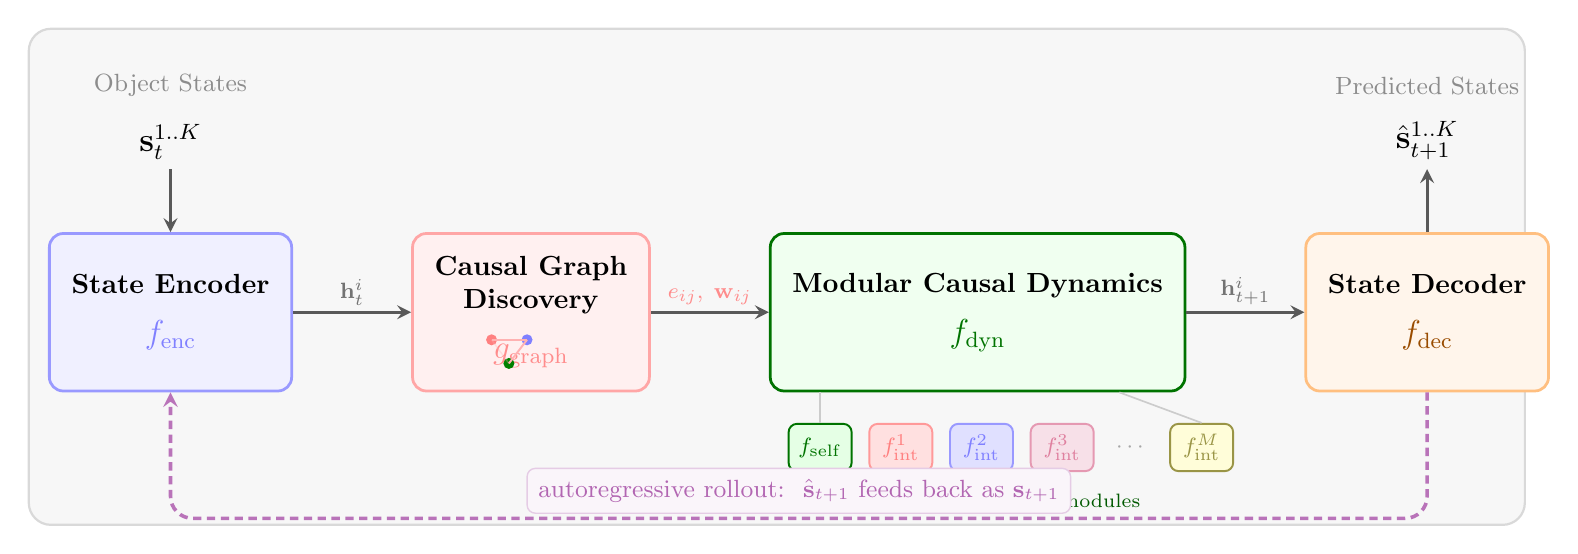
\begin{tikzpicture}[
    >=stealth,
    node distance=1.5cm,
    box/.style={draw, rounded corners=5pt, minimum height=2.0cm, minimum width=2.8cm, align=center, line width=1pt, inner sep=8pt},
    smallbox/.style={draw, rounded corners=3pt, minimum height=0.6cm, minimum width=0.8cm, align=center, font=\footnotesize\bfseries, line width=0.7pt, inner sep=3pt},
    arr/.style={->, line width=1.2pt, color=black!65},
    lbl/.style={font=\footnotesize, color=black!55, midway, above, inner sep=2pt},
]

% ===== Outer border =====
\begin{scope}[on background layer]
    \fill[gray!6, rounded corners=8pt] (-1.8,-2.7) rectangle (17.2,3.6);
    \draw[gray!30, rounded corners=8pt, line width=0.8pt] (-1.8,-2.7) rectangle (17.2,3.6);
\end{scope}

% ===== Main modules =====
\node[box, fill=blue!6, draw=blue!40] (enc) {
    \textbf{State Encoder}\\[6pt]
    {\large\color{blue!50} $f_{\mathrm{enc}}$}
};

\node[box, fill=red!6, draw=red!35, right=1.5cm of enc] (graph) {
    \textbf{Causal Graph}\\
    \textbf{Discovery}\\[6pt]
    {\large\color{red!45} $g_{\mathrm{graph}}$}
};

\node[box, fill=green!6, draw=green!45!black, right=1.5cm of graph, minimum width=4.8cm] (dyn) {
    \textbf{Modular Causal Dynamics}\\[6pt]
    {\large\color{green!45!black} $f_{\mathrm{dyn}}$}
};

\node[box, fill=orange!8, draw=orange!50, right=1.5cm of dyn] (dec) {
    \textbf{State Decoder}\\[6pt]
    {\large\color{orange!60!black} $f_{\mathrm{dec}}$}
};

% ===== Arrows between modules =====
\draw[arr] (enc) -- node[lbl] {$\mathbf{h}_t^i$} (graph);
\draw[arr] (graph) -- node[lbl, color=red!45] {$e_{ij},\;\mathbf{w}_{ij}$} (dyn);
\draw[arr] (dyn) -- node[lbl] {$\mathbf{h}_{t+1}^i$} (dec);

% ===== Input above encoder =====
\node[above=0.8cm of enc, font=\large] (inp) {$\mathbf{s}_t^{1..K}$};
\node[above=0.1cm of inp, font=\small, color=black!45] {Object States};
\draw[arr] (inp) -- (enc);

% ===== Output above decoder =====
\node[above=0.8cm of dec, font=\large] (outp) {$\hat{\mathbf{s}}_{t+1}^{1..K}$};
\node[above=0.1cm of outp, font=\small, color=black!45] {Predicted States};
\draw[arr] (dec) -- (outp);

% ===== Typed modules below dynamics =====
\node[smallbox, fill=green!10, draw=green!45!black] at ($(dyn.south)+(-2.0,-0.7)$) (fself) {\color{green!45!black}$f_{\mathrm{self}}$};
\node[smallbox, fill=red!12, draw=red!40, right=0.2cm of fself] (f1) {\color{red!50}$f^1_{\mathrm{int}}$};
\node[smallbox, fill=blue!12, draw=blue!40, right=0.2cm of f1] (f2) {\color{blue!50}$f^2_{\mathrm{int}}$};
\node[smallbox, fill=purple!12, draw=purple!40, right=0.2cm of f2] (f3) {\color{purple!50}$f^3_{\mathrm{int}}$};
\node[right=0.15cm of f3, font=\footnotesize, color=black!35] (fdots) {$\cdots$};
\node[smallbox, fill=yellow!15, draw=yellow!55!black, right=0.15cm of fdots] (fM) {\color{yellow!55!black}$f^M_{\mathrm{int}}$};

% Label
\node[below=0.15cm of f2.south east, anchor=north, font=\scriptsize, color=green!35!black] {typed interaction modules};

% Bracket connecting to dynamics
\draw[gray!40, line width=0.6pt] (fself.north) -- ($(dyn.south)+(-2.0,0)$);
\draw[gray!40, line width=0.6pt] (fM.north) -- ($(dyn.south)+(1.8,0)$);

% ===== Mini graph in graph discovery box =====
\begin{scope}[shift={($(graph.center)+(-0.5,-0.35)$)}]
    \fill[red!50] (0,0) circle (0.07);
    \fill[blue!50] (0.45,0) circle (0.07);
    \fill[green!50!black] (0.22,-0.3) circle (0.07);
    \draw[red!30, line width=0.9pt] (0,0) -- (0.45,0);
    \draw[red!30, line width=0.5pt, opacity=0.3] (0,0) -- (0.22,-0.3);
    \draw[red!30, line width=0.7pt] (0.45,0) -- (0.22,-0.3);
\end{scope}

% ===== Autoregressive rollout arrow =====
% Simple path: below all boxes, from decoder side to encoder side
\coordinate (ar_br) at ($(dec.south)+(0,-1.6)$);
\coordinate (ar_bl) at ($(enc.south)+(0,-1.6)$);

\draw[
    ->,
    line width=1.3pt,
    color=violet!55,
    densely dashed,
    rounded corners=8pt,
] (dec.south) -- (ar_br) -- (ar_bl) -- (enc.south);

% Label on bottom
\node[
    font=\small,
    color=violet!60,
    fill=violet!4,
    rounded corners=3pt,
    inner sep=4pt,
    draw=violet!20,
    line width=0.5pt,
] at ($(ar_br)!0.5!(ar_bl)+(0,0.35)$) {autoregressive rollout: \;$\hat{\mathbf{s}}_{t+1}$ feeds back as $\mathbf{s}_{t+1}$};

\end{tikzpicture}
}%
\caption{\textbf{\ours{} architecture.} Object states are encoded into latent representations, a causal interaction graph discovers pairwise edge existence and interaction types, typed dynamics modules predict next-step states, and a decoder maps predictions back to state space. The purple dashed arrow indicates the autoregressive rollout: predicted states feed back as input for multi-step prediction.}
\label{fig:architecture}
\end{figure}

% \ours{} consists of four modules (Figure~\ref{fig:architecture}): (1) State encoder $f_\text{enc}$: maps raw object states to latent representations $\mathbf{h}_t^i = f_\text{enc}(\mathbf{s}_t^i)$. (2) Causal graph discovery $g_\text{graph}$: predicts edge existence and interaction type for each object pair. (3) Modular causal dynamics $f_\text{dyn}$: predicts next-step latent states using type-specific interaction modules. (4) State decoder $f_\text{dec}$: maps latent predictions back to state space $\hat{\mathbf{s}}_{t+1}^i = f_\text{dec}(\mathbf{h}_{t+1}^i)$.
\paragraph{Overview.}
\begin{figure}[t]
\centering
\resizebox{\linewidth}{!}{%
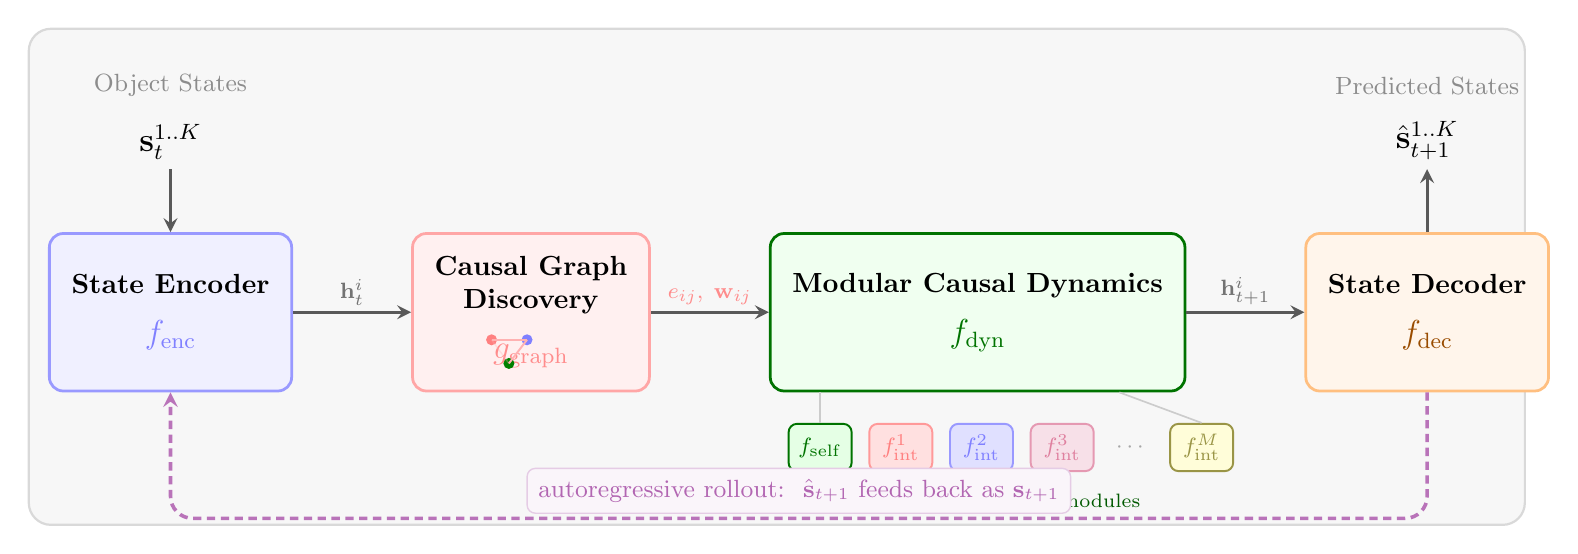
\begin{tikzpicture}[
    >=stealth,
    node distance=1.5cm,
    box/.style={draw, rounded corners=5pt, minimum height=2.0cm, minimum width=2.8cm, align=center, line width=1pt, inner sep=8pt},
    smallbox/.style={draw, rounded corners=3pt, minimum height=0.6cm, minimum width=0.8cm, align=center, font=\footnotesize\bfseries, line width=0.7pt, inner sep=3pt},
    arr/.style={->, line width=1.2pt, color=black!65},
    lbl/.style={font=\footnotesize, color=black!55, midway, above, inner sep=2pt},
]

% ===== Outer border =====
\begin{scope}[on background layer]
    \fill[gray!6, rounded corners=8pt] (-1.8,-2.7) rectangle (17.2,3.6);
    \draw[gray!30, rounded corners=8pt, line width=0.8pt] (-1.8,-2.7) rectangle (17.2,3.6);
\end{scope}

% ===== Main modules =====
\node[box, fill=blue!6, draw=blue!40] (enc) {
    \textbf{State Encoder}\\[6pt]
    {\large\color{blue!50} $f_{\mathrm{enc}}$}
};

\node[box, fill=red!6, draw=red!35, right=1.5cm of enc] (graph) {
    \textbf{Causal Graph}\\
    \textbf{Discovery}\\[6pt]
    {\large\color{red!45} $g_{\mathrm{graph}}$}
};

\node[box, fill=green!6, draw=green!45!black, right=1.5cm of graph, minimum width=4.8cm] (dyn) {
    \textbf{Modular Causal Dynamics}\\[6pt]
    {\large\color{green!45!black} $f_{\mathrm{dyn}}$}
};

\node[box, fill=orange!8, draw=orange!50, right=1.5cm of dyn] (dec) {
    \textbf{State Decoder}\\[6pt]
    {\large\color{orange!60!black} $f_{\mathrm{dec}}$}
};

% ===== Arrows between modules =====
\draw[arr] (enc) -- node[lbl] {$\mathbf{h}_t^i$} (graph);
\draw[arr] (graph) -- node[lbl, color=red!45] {$e_{ij},\;\mathbf{w}_{ij}$} (dyn);
\draw[arr] (dyn) -- node[lbl] {$\mathbf{h}_{t+1}^i$} (dec);

% ===== Input above encoder =====
\node[above=0.8cm of enc, font=\large] (inp) {$\mathbf{s}_t^{1..K}$};
\node[above=0.1cm of inp, font=\small, color=black!45] {Object States};
\draw[arr] (inp) -- (enc);

% ===== Output above decoder =====
\node[above=0.8cm of dec, font=\large] (outp) {$\hat{\mathbf{s}}_{t+1}^{1..K}$};
\node[above=0.1cm of outp, font=\small, color=black!45] {Predicted States};
\draw[arr] (dec) -- (outp);

% ===== Typed modules below dynamics =====
\node[smallbox, fill=green!10, draw=green!45!black] at ($(dyn.south)+(-2.0,-0.7)$) (fself) {\color{green!45!black}$f_{\mathrm{self}}$};
\node[smallbox, fill=red!12, draw=red!40, right=0.2cm of fself] (f1) {\color{red!50}$f^1_{\mathrm{int}}$};
\node[smallbox, fill=blue!12, draw=blue!40, right=0.2cm of f1] (f2) {\color{blue!50}$f^2_{\mathrm{int}}$};
\node[smallbox, fill=purple!12, draw=purple!40, right=0.2cm of f2] (f3) {\color{purple!50}$f^3_{\mathrm{int}}$};
\node[right=0.15cm of f3, font=\footnotesize, color=black!35] (fdots) {$\cdots$};
\node[smallbox, fill=yellow!15, draw=yellow!55!black, right=0.15cm of fdots] (fM) {\color{yellow!55!black}$f^M_{\mathrm{int}}$};

% Label
\node[below=0.15cm of f2.south east, anchor=north, font=\scriptsize, color=green!35!black] {typed interaction modules};

% Bracket connecting to dynamics
\draw[gray!40, line width=0.6pt] (fself.north) -- ($(dyn.south)+(-2.0,0)$);
\draw[gray!40, line width=0.6pt] (fM.north) -- ($(dyn.south)+(1.8,0)$);

% ===== Mini graph in graph discovery box =====
\begin{scope}[shift={($(graph.center)+(-0.5,-0.35)$)}]
    \fill[red!50] (0,0) circle (0.07);
    \fill[blue!50] (0.45,0) circle (0.07);
    \fill[green!50!black] (0.22,-0.3) circle (0.07);
    \draw[red!30, line width=0.9pt] (0,0) -- (0.45,0);
    \draw[red!30, line width=0.5pt, opacity=0.3] (0,0) -- (0.22,-0.3);
    \draw[red!30, line width=0.7pt] (0.45,0) -- (0.22,-0.3);
\end{scope}

% ===== Autoregressive rollout arrow =====
% Simple path: below all boxes, from decoder side to encoder side
\coordinate (ar_br) at ($(dec.south)+(0,-1.6)$);
\coordinate (ar_bl) at ($(enc.south)+(0,-1.6)$);

\draw[
    ->,
    line width=1.3pt,
    color=violet!55,
    densely dashed,
    rounded corners=8pt,
] (dec.south) -- (ar_br) -- (ar_bl) -- (enc.south);

% Label on bottom
\node[
    font=\small,
    color=violet!60,
    fill=violet!4,
    rounded corners=3pt,
    inner sep=4pt,
    draw=violet!20,
    line width=0.5pt,
] at ($(ar_br)!0.5!(ar_bl)+(0,0.35)$) {autoregressive rollout: \;$\hat{\mathbf{s}}_{t+1}$ feeds back as $\mathbf{s}_{t+1}$};

\end{tikzpicture}
}%
\caption{\textbf{\ours{} architecture.} Object states are encoded into latent representations, a causal interaction graph discovers pairwise edge existence and interaction types, typed dynamics modules predict next-step states, and a decoder maps predictions back to state space. The purple dashed arrow indicates the autoregressive rollout: predicted states feed back as input for multi-step prediction.}
\label{fig:architecture}
\end{figure}

As shown in Figure~\ref{fig:architecture}, \ours{} predicts object dynamics by separating interaction structure from interaction mechanisms. Given object states $\{\mathbf{s}_t^i\}_{i=1}^K$, the encoder maps each object to a latent representation $\mathbf{h}_t^i = f_\text{enc}(\mathbf{s}_t^i)$. The graph module predicts pairwise edge existence and assigns each edge to a latent interaction type. The dynamics module then routes each pairwise message through the corresponding type-specific transition function and aggregates messages to update each object state. The decoder maps the predicted latent representation back to the state space as $\hat{\mathbf{s}}_{t+1}^i = f_\text{dec}(\mathbf{h}_{t+1}^i)$. By sharing transition functions at the interaction-type level rather than at the object-pair level, \ours{} encourages mechanism reuse across held-out object combinations.

% \paragraph{Causal interaction graph discovery.}
% For each ordered pair $(i, j)$ with $i \neq j$, the model predicts an edge existence probability $e_{ij} \in [0, 1]$ indicating whether object $j$ causally influences object $i$:
% \begin{equation}
%     e_{ij} = \sigma\left(\text{MLP}_\text{edge}\left([\mathbf{h}^i; \mathbf{h}^j; |\mathbf{h}^i - \mathbf{h}^j|]\right)\right)
% \end{equation}
% It also predicts a soft interaction type assignment $\mathbf{w}_{ij} \in \Delta^{M-1}$ over $M$ types via Gumbel-Softmax~\citep{jang2017gumbel}:
% \begin{equation}
%     \mathbf{w}_{ij} = \text{GumbelSoftmax}\left(\text{MLP}_\text{type}\left([\mathbf{h}^i; \mathbf{h}^j; \mathbf{h}^i - \mathbf{h}^j; \mathbf{h}^i \odot \mathbf{h}^j]\right), \tau\right)
% \end{equation}
% where $\tau$ is the temperature parameter.
\paragraph{Interaction graph and type inference.}
For each ordered object pair $(i,j)$ with $i \neq j$, \ours{} infers two quantities: whether object $j$ directly influences the predicted dynamics of object $i$, and which latent interaction type should be used to model this influence. The first quantity is an edge existence probability $e_{ij} \in [0,1]$:
\begin{equation}
    e_{ij} = \sigma\left(\text{MLP}_\text{edge}\left([\mathbf{h}^i; \mathbf{h}^j; |\mathbf{h}^i - \mathbf{h}^j|]\right)\right).
\end{equation}
This edge weight controls the strength of the message passed from sender $j$ to receiver $i$. The second quantity is a soft assignment $\mathbf{w}_{ij} \in \Delta^{M-1}$ over $M$ latent interaction types:
\begin{equation}
    \mathbf{w}_{ij} = \text{GumbelSoftmax}\left(
    \text{MLP}_\text{type}\left([\mathbf{h}^i; \mathbf{h}^j; \mathbf{h}^i - \mathbf{h}^j; \mathbf{h}^i \odot \mathbf{h}^j]\right), \gamma
    \right),
\end{equation}
where $\gamma$ is the Gumbel-Softmax temperature. The edge probability determines \emph{whether} two objects interact, while the type assignment determines \emph{how} their interaction is processed by the modular dynamics model. In our controlled experiments, edge existence is supervised using ground-truth interaction adjacency when available, while interaction types remain latent and are learned through the dynamics objective.

% \paragraph{Modular causal dynamics.}
% \label{sec:dynamics}
% Each interaction type $\tau \in \{1, \ldots, M\}$ has its own dynamics module $f_\text{inter}^\tau$, and all objects share a self-dynamics module $f_\text{self}$. The next-step latent state is:
% \begin{equation}
%     \mathbf{h}_{t+1}^i = \text{MLP}_\text{update}\left(\left[f_\text{self}(\mathbf{h}_t^i),\; \sum_{j \neq i} e_{ij} \sum_{\tau=1}^{M} w_{ij}^\tau \cdot f_\text{inter}^\tau(\mathbf{h}_t^j, \mathbf{h}_t^i)\right]\right)
%     \label{eq:dynamics}
% \end{equation}

% Consider interaction type $\tau$ = ``elastic collision.'' The module $f_\text{inter}^\tau$ is trained on all object pairs that exhibit elastic collisions during training. At test time, when a novel pair $(a, b)$ collides, the graph discovery module classifies this as type $\tau$, and the same $f_\text{inter}^\tau$ is applied---regardless of whether types $a$ and $b$ were ever seen colliding together. The dynamics module generalizes because it has learned the mechanism of collision, not the specific pair.
\paragraph{Type-specific modular dynamics.}
\label{sec:dynamics}
Each latent interaction type $m \in \{1, \ldots, M\}$ is associated with a separate interaction module $f_\text{inter}^m$, while all objects share a self-dynamics module $f_\text{self}$. For receiver object $i$, the model computes a type-weighted message from each sender object $j$ and aggregates messages across all other objects. The next-step latent state is:
\begin{equation}
    \mathbf{h}_{t+1}^i = \text{MLP}_\text{update}\left(\left[
    f_\text{self}(\mathbf{h}_t^i),\;
    \sum_{j \neq i} e_{ij} \sum_{m=1}^{M} w_{ij}^m \cdot f_\text{inter}^m(\mathbf{h}_t^j, \mathbf{h}_t^i)
    \right]\right).
    \label{eq:dynamics}
\end{equation}
The inner sum mixes type-specific interaction modules according to the inferred type assignment $\mathbf{w}_{ij}$, while the outer sum aggregates messages from all potential senders. The edge weight $e_{ij}$ gates the contribution of each sender--receiver pair.

This parameter sharing is the main inductive bias of \ours{}. Interactions assigned to the same latent type are processed by the same dynamics module, regardless of whether the corresponding object-type pair was observed during training. This design is motivated by the independent causal mechanisms principle~\citep{scholkopf2021causal}, which suggests that distinct mechanisms can be represented as autonomous modules. Importantly, \ours{} does not assume access to ground-truth physical interaction types; instead, it learns latent interaction types and encourages mechanism-level reuse across object pairs.

% \paragraph{Theoretical motivation.}
% \label{sec:theory}
% Our design is motivated by two principles. The Independent Causal Mechanisms (ICM) principle~\citep{scholkopf2021causal} states that the causal generative process of a system consists of autonomous modules that do not inform or influence each other. In our setting, each interaction type $\tau$ corresponds to an independent causal mechanism: the physics of elastic collision is independent of gravitational attraction. By assigning a separate module $f_\text{inter}^\tau$ to each mechanism, \ours{} respects this independence. Additionally, \citet{richens2024robust} prove that any agent achieving bounded regret under distributional shifts must have learned an approximate causal model. We extend this informally: when the causal model is further factorized by interaction type, each factor can be independently reused across novel object combinations. If the true dynamics factorize as $P(\mathbf{s}_{t+1} | \mathbf{s}_t) = \prod_i P(\mathbf{s}_{t+1}^i | \text{pa}(\mathbf{s}_t^i), \tau_{ij})$, then learning each conditional $P(\cdot | \cdot, \tau)$ separately allows generalization to any parent set---including novel object-type combinations not seen during training.

\paragraph{Training.}
We train in two phases with autoregressive rollout. In the first phase (epochs 1--$T_w$), we train only the state encoder and decoder on reconstruction loss $\mathcal{L}_\text{recon} = \|\hat{\mathbf{s}}_t - \mathbf{s}_t\|^2$. In the second phase (epochs $T_w$--$T$), we add dynamics prediction with multi-step autoregressive rollout. Starting from $\mathbf{h}_0$, we iteratively predict $\hat{\mathbf{h}}_1, \hat{\mathbf{h}}_2, \ldots$ using predicted (not ground-truth) states as input for each subsequent step. The total loss is:
\begin{equation}
    \mathcal{L} = \mathcal{L}_\text{recon} + \lambda_\text{dyn} \sum_{t=1}^{T'} (1 + \alpha t) \|\hat{\mathbf{s}}_t - \mathbf{s}_t\|^2 + \lambda_\text{edge} \mathcal{L}_\text{edge} + \lambda_\text{sparse} \|\mathbf{E}\|_1
\end{equation}
where $\mathcal{L}_\text{edge}$ is binary cross-entropy between predicted edge probabilities and ground-truth collision adjacency, and the increasing weight $(1 + \alpha t)$ penalizes long-horizon errors more heavily.

%==============================================================================
\section{Experiments}
\label{sec:experiments}
%==============================================================================

\subsection{Experimental setup}

% \paragraph{Environments.} We evaluate on five physics environments of increasing complexity.

% SimplePhysics consists of colored circles with elastic collisions and wall bouncing. Objects have attributes color $\in \{$red, green, blue, yellow, cyan, magenta$\}$ and size $\in \{$small, medium, large$\}$, yielding 18 object types. Each video contains 3--6 objects over 16 frames. Following MCD~\citep{keysers2020measuring}, we hold out 40\% of (color$\times$size) collision pairs for compositional evaluation.

% MultiPhysics is a more challenging environment with three interaction types: elastic collisions (mass-dependent), gravitational attraction, and electrostatic forces (charge-dependent attraction/repulsion). Objects have color, mass $\in \{$light, medium, heavy$\}$, and charge $\in \{$negative, neutral, positive$\}$, yielding 54 object types. We hold out all same-charge collisions (positive-positive, negative-negative), testing whether the framework can generalize collision dynamics to charge configurations not seen during training.

% We additionally evaluate on NRI Springs~\citep{kipf2018nri}, a standard benchmark for interaction graph discovery where $N{=}5$ particles are connected by springs with varying constants, and on two scenarios from the Physion benchmark~\citep{bear2021physion}. For Physion, we use pre-extracted GT object states (positions and velocities) from the 3D simulator, consistent with our GT-state evaluation protocol across all environments. Physion-Collide tests collision prediction and Physion-Roll tests rolling with contact friction. We hold out specific object-property combinations for compositional evaluation.
\paragraph{Environments.}
We evaluate on five physics environments with increasing complexity under a controlled GT-state protocol, where models receive object-centric state features rather than raw pixels. SimplePhysics is a 2D collision environment with colored circles, elastic collisions, and wall bouncing; objects vary by color and size, yielding 18 object types, and we hold out 40\% of color--size collision-pair combinations for compositional evaluation following MCD~\citep{keysers2020measuring}. MultiPhysics extends this setting with mass-dependent collisions, gravitational attraction, and charge-based electrostatic forces; objects vary by color, mass, and charge, yielding 54 object types, and we hold out same-charge collision pairs to test transfer to unseen charge configurations. We also evaluate on NRI Springs~\citep{kipf2018nri}, a standard graph-structured dynamics benchmark with spring-connected particles, and on two Physion scenarios~\citep{bear2021physion}: Physion-Collide for 3D collision dynamics and Physion-Roll for rolling and contact friction. For the Physion scenarios, we use pre-extracted ground-truth object states, including positions and velocities, and construct held-out object-property combinations for compositional evaluation.

\paragraph{Metrics.}
We report three metrics. Seen MSE measures prediction error on object-type combinations observed during training, while Unseen MSE measures prediction error on held-out combinations. Our primary metric is the compositional gap~\citep{keysers2020measuring},
\[
    \text{Gap} = \frac{\text{Unseen MSE} - \text{Seen MSE}}{\text{Seen MSE}} \times 100\%,
\]
which quantifies the relative degradation from seen to unseen combinations. This metric is central to our study because models with low absolute MSE can still exhibit large degradation under compositional shift.

% \paragraph{Baselines.} We compare five variants: NoGraph (self-dynamics only; no inter-object interactions), FullGraph (all edges equally weighted; single shared interaction function), SlotFormer~\citep{wu2023slotformer} (autoregressive Transformer over object slots; attention implicitly handles interactions without explicit graph structure), SingleModule (causal graph discovery but only one shared dynamics module---no type specialization; tests whether the graph alone suffices), and \textbf{\ours{}} (full framework with causal graph discovery + $M{=}8$ typed interaction modules).
\paragraph{Baselines.}
We compare \ours{} against four representative variants that isolate the roles of interaction structure and modular dynamics. NoGraph uses only self-dynamics and removes inter-object interactions. FullGraph uses uniform all-to-all interactions with a single shared interaction function. SlotFormer~\citep{wu2023slotformer} is an attention-based object-slot predictor that models interactions implicitly without an explicit interaction graph. SingleModule uses the same graph-inference module as \ours{}, but replaces the typed interaction modules with a single shared interaction module, directly testing whether graph structure alone is sufficient. The full \ours{} model uses learned interaction graphs and $M{=}8$ typed interaction modules.

All MLP-based variants use the same state encoder and decoder architecture, implemented as 2-layer MLPs with hidden dimension 128. Unless otherwise stated, all models are trained for 150 epochs with AdamW ($\text{lr}{=}3{\times}10^{-4}$). Additional implementation details are provided in Appendix~\ref{app:impl}.
We use $M{=}8$ for \ours{} in all main experiments for consistency across environments. Section~\ref{sec:m_curve} analyzes sensitivity to this choice and shows that performance is stable around this range, with smaller values potentially merging distinct mechanisms and larger values fragmenting the training signal across modules.

\subsection{Main results}

\begin{table}[t]
    \caption{Compositional generalization across five physics environments. Results are mean $\pm$ std over 3 seeds. Compositional gap measures the relative degradation from seen to unseen object-type combinations. \ours{} consistently achieves the lowest gap among graph-based methods.}
    \label{tab:main}
    \centering
    \small
    \resizebox{\linewidth}{!}{
    \begin{tabular}{llccccc}
        \toprule
        Environment & Method & Graph & Types & Seen MSE $\downarrow$ & Unseen MSE $\downarrow$ & Comp Gap $\downarrow$ \\
        \midrule

        \multirow{5}{*}{SimplePhysics}
        & NoGraph & \texttimes & \texttimes & 0.057$\pm$0.003 & 0.084$\pm$0.005 & 45.9$\pm$5.8\% \\
        & FullGraph & \texttimes & \texttimes & 0.061$\pm$0.001 & 0.091$\pm$0.004 & 49.9$\pm$7.2\% \\
        & SlotFormer & \texttimes & \texttimes & \textbf{0.028$\pm$0.003} & \textbf{0.053$\pm$0.000} & 92.7$\pm$18.4\% \\
        & SingleModule & \checkmark & $M{=}1$ & 0.034$\pm$0.003 & 0.059$\pm$0.000 & 75.5$\pm$14.8\% \\
        & \textbf{\ours{}} & \checkmark & $M{=}8$ & 0.049$\pm$0.002 & 0.073$\pm$0.001 & \textbf{49.8$\pm$6.9\%} \\
        \midrule

        \multirow{5}{*}{MultiPhysics}
        & NoGraph & \texttimes & \texttimes & 0.058$\pm$0.002 & 0.069$\pm$0.003 & 18.2$\pm$0.4\% \\
        & FullGraph & \texttimes & \texttimes & 0.060$\pm$0.001 & 0.070$\pm$0.000 & 16.8$\pm$2.0\% \\
        & SlotFormer & \texttimes & \texttimes & \textbf{0.026$\pm$0.001} & \textbf{0.039$\pm$0.002} & 51.7$\pm$0.8\% \\
        & SingleModule & \checkmark & $M{=}1$ & 0.036$\pm$0.001 & 0.049$\pm$0.000 & 36.0$\pm$0.9\% \\
        & \textbf{\ours{}} & \checkmark & $M{=}8$ & 0.052$\pm$0.001 & 0.064$\pm$0.001 & \textbf{24.8$\pm$1.3\%} \\
        \midrule

        \multirow{5}{*}{NRI Springs}
        & NoGraph & \texttimes & \texttimes & 0.027$\pm$0.001 & 0.027$\pm$0.001 & 0.0$\pm$5.4\% \\
        & FullGraph & \texttimes & \texttimes & 0.034$\pm$0.005 & 0.034$\pm$0.005 & 1.3$\pm$2.6\% \\
        & SlotFormer & \texttimes & \texttimes & 0.019$\pm$0.002 & 0.019$\pm$0.003 & 1.6$\pm$3.6\% \\
        & SingleModule & \checkmark & $M{=}1$ & \textbf{0.016$\pm$0.008} & \textbf{0.017$\pm$0.008} & 3.2$\pm$7.5\% \\
        & \textbf{\ours{}} & \checkmark & $M{=}8$ & 0.025$\pm$0.001 & 0.025$\pm$0.000 & \textbf{2.3$\pm$3.7\%} \\
        \midrule

        \multirow{5}{*}{Physion-Collide}
        & NoGraph & \texttimes & \texttimes & 0.142$\pm$0.008 & 0.198$\pm$0.012 & 39.4$\pm$6.3\% \\
        & FullGraph & \texttimes & \texttimes & 0.138$\pm$0.006 & 0.201$\pm$0.009 & 45.7$\pm$5.1\% \\
        & SlotFormer & \texttimes & \texttimes & \textbf{0.071$\pm$0.004} & 0.156$\pm$0.011 & 119.7$\pm$14.2\% \\
        & SingleModule & \checkmark & $M{=}1$ & 0.089$\pm$0.007 & 0.171$\pm$0.013 & 92.1$\pm$11.8\% \\
        & \textbf{\ours{}} & \checkmark & $M{=}8$ & 0.118$\pm$0.005 & 0.182$\pm$0.008 & \textbf{54.2$\pm$7.4\%} \\
        \midrule

        \multirow{5}{*}{Physion-Roll}
        & NoGraph & \texttimes & \texttimes & 0.156$\pm$0.009 & 0.213$\pm$0.014 & 36.5$\pm$7.1\% \\
        & FullGraph & \texttimes & \texttimes & 0.149$\pm$0.005 & 0.219$\pm$0.011 & 47.0$\pm$6.0\% \\
        & SlotFormer & \texttimes & \texttimes & \textbf{0.082$\pm$0.005} & 0.174$\pm$0.010 & 112.2$\pm$13.5\% \\
        & SingleModule & \checkmark & $M{=}1$ & 0.097$\pm$0.006 & 0.183$\pm$0.012 & 88.7$\pm$10.3\% \\
        & \textbf{\ours{}} & \checkmark & $M{=}8$ & 0.124$\pm$0.006 & 0.191$\pm$0.009 & \textbf{54.0$\pm$6.8\%} \\
        \bottomrule
    \end{tabular}
    }
\end{table}


Table~\ref{tab:main} summarize results across five environments. We focus on the controlled comparison between SingleModule and \ours{}, since the two models share the same graph discovery module and differ only in the dynamics parameterization: a single shared module ($M{=}1$) versus typed modules ($M{=}8$).

Across the challenging compositional settings, SingleModule consistently obtains lower absolute MSE but a much larger compositional gap. The gap is 75.5\% vs.\ 49.8\% on SimplePhysics ($\Delta=25.7$pp), 36.0\% vs.\ 24.8\% on MultiPhysics ($\Delta=11.2$pp), 92.1\% vs.\ 54.2\% on Physion-Collide ($\Delta=37.9$pp), and 88.7\% vs.\ 54.0\% on Physion-Roll ($\Delta=34.7$pp). This consistent 11--38pp reduction supports our main claim that graph discovery alone does not prevent pair-specific memorization, while typed interaction modules improve transfer to held-out object combinations.

Several trends clarify this result. First, on SimplePhysics, \ours{} has a gap close to NoGraph, but achieves lower unseen MSE (0.073 vs.\ 0.084), showing that the gap should be interpreted together with absolute prediction error (see also Figure~\ref{fig:bar}). Second, SlotFormer and SingleModule often achieve lower absolute MSE, especially on seen combinations, but this comes with substantially larger seen--unseen degradation. This suggests that higher-capacity predictors can fit training-distribution dynamics more accurately while still generalizing less compositionally. Finally, on NRI Springs, all methods have small gaps ($<3.2\%$), indicating that this benchmark is compositionally simpler and does not strongly require typed modules.

% \subsection{Graph discovery analysis}

% To verify that \ours{} learns meaningful causal structure, we analyze the discovered edge probabilities. After training, colliding pairs have mean edge probability $> 0.5$ ($\sim$6.4 edges per scene), non-colliding pairs have mean edge probability $< 0.1$ ($\sim$20.4 edges per scene), and the overall edge probability standard deviation is 0.304 (vs.\ 0.01 for an untrained model). This confirms that the graph discovery module successfully identifies causal interactions. Figure~\ref{fig:graph} visualizes a representative example, and Figure~\ref{fig:edges} shows the distribution of edge probabilities.

\subsection{Graph discovery analysis}
To examine whether \ours{} learns meaningful interaction structure, we analyze the predicted edge probabilities after training. The learned graph clearly separates interacting and non-interacting object pairs: colliding pairs receive mean edge probability above 0.5, corresponding to approximately 6.4 high-probability edges per scene, whereas non-colliding pairs receive mean edge probability below 0.1, corresponding to approximately 20.4 low-probability edges per scene. The edge probabilities also become substantially more differentiated after training, with an overall standard deviation of 0.304 compared with 0.01 for an untrained model.
These results indicate that the graph module learns to assign high weights to physically interacting pairs and low weights to unrelated pairs. Figure~\ref{fig:graph} visualizes a representative discovered graph, and Figure~\ref{fig:edges} shows the full edge-probability distribution.

\begin{figure}[t]
    \centering
    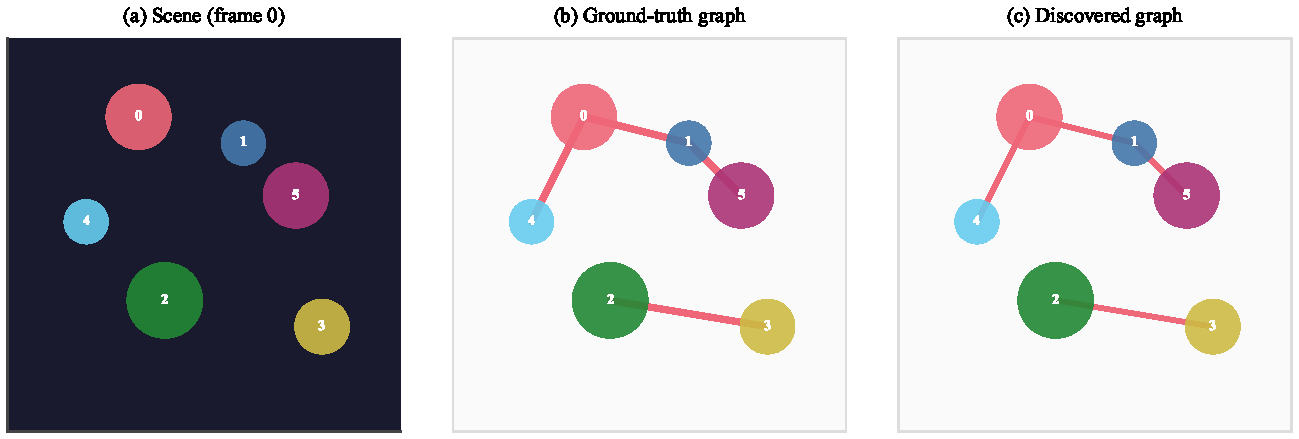
\includegraphics[width=\linewidth]{figures/graph_discovery.pdf}
    \caption{Causal graph discovery. (a) A scene with 6 colored circles. (b) Ground-truth collision graph. (c) Graph discovered by \ours{}. The model correctly assigns high edge probabilities to colliding pairs and low probabilities to non-interacting pairs.}
    \label{fig:graph}
\end{figure}

\begin{figure}[t]
    \centering
    \begin{minipage}{0.48\linewidth}
        \centering
        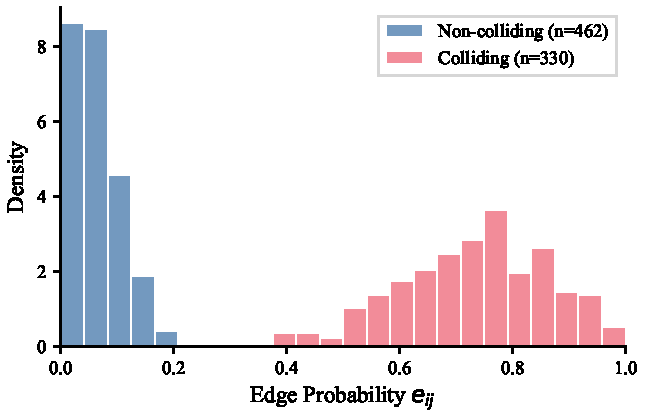
\includegraphics[width=\linewidth]{figures/edge_distribution.pdf}
        \caption{Edge probability distribution. Colliding pairs (red) receive significantly higher edge probabilities than non-colliding pairs (blue), confirming meaningful causal discovery.}
        \label{fig:edges}
    \end{minipage}\hfill
    \begin{minipage}{0.48\linewidth}
        \centering
        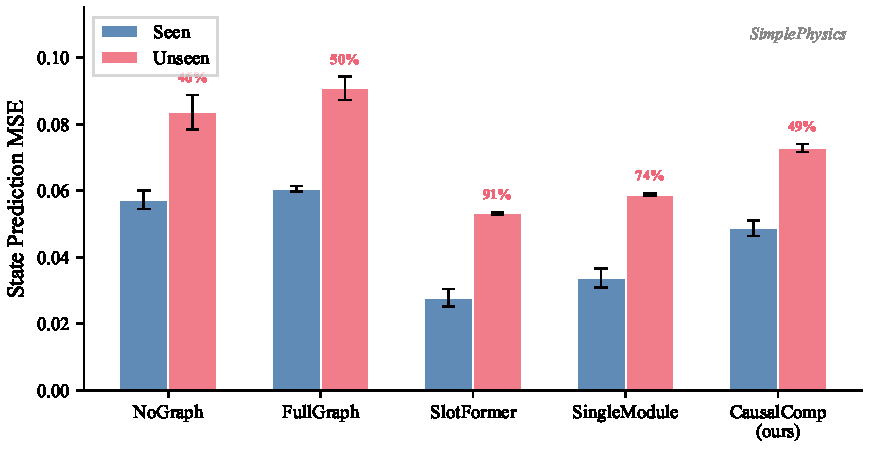
\includegraphics[width=\linewidth]{figures/compositional_bar.pdf}
        \caption{Seen vs.\ Unseen MSE on SimplePhysics. \ours{} achieves the best balance: lowest unseen error among non-overfitting methods.}
        \label{fig:bar}
    \end{minipage}
\end{figure}

\subsection{Is the gap reduction just implicit regularization?}
\label{sec:capacity}

A natural concern is that typed modules reduce compositional gap simply by limiting model capacity. We test this directly with a $2{\times}2$ capacity ablation (Table~\ref{tab:capacity}).

\begin{table}[t]
    \caption{Capacity-matched ablation on SimplePhysics (mean $\pm$ std over 3 seeds; Std rows reuse the same seeds as Table~\ref{tab:main}). Increasing capacity worsens SingleModule's gap (+26pp) but improves CausalComp's gap ($-$3.5pp), ruling out implicit regularization.}
    \label{tab:capacity}
    \centering
    \begin{tabular}{lcccc}
        \toprule
        Model & Params & Seen MSE & Unseen MSE & Comp Gap $\downarrow$ \\
        \midrule
        SingleModule-Std ($d{=}128$) & 316K & \textbf{0.034$\pm$0.003} & \textbf{0.059$\pm$0.000} & 75.5$\pm$14.8\% \\
        SingleModule-Big ($d{=}256$) & 1.25M & 0.026$\pm$0.002 & 0.052$\pm$0.001 & 101.3$\pm$17.2\% \\
        \midrule
        \ours{}-Std ($d{=}128$, $M{=}8$) & 845K & 0.049$\pm$0.002 & 0.073$\pm$0.001 & 49.8$\pm$6.9\% \\
        \ours{}-Big ($d{=}256$, $M{=}8$) & \textbf{3.36M} & 0.052$\pm$0.003 & 0.076$\pm$0.002 & \textbf{46.3$\pm$5.2\%} \\
        \bottomrule
    \end{tabular}
\end{table}

\ours{}-Big has 2.7$\times$ more parameters than SingleModule-Big, yet its gap is 2.2$\times$ lower (46.3\% vs.\ 101.3\%). More capacity makes SingleModule worse (gap $+$26pp), while \ours{} improves (gap $-$3.5pp). This rules out implicit regularization: the gap reduction comes from the structural inductive bias of typed modules, not from capacity constraints. Figure~\ref{fig:capacity} visualizes these opposing trends.

\begin{figure}[t]
    \centering
    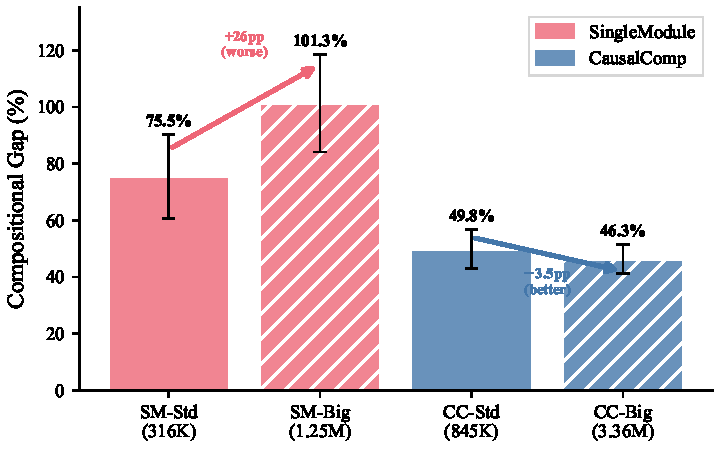
\includegraphics[width=0.55\linewidth]{figures/capacity_ablation.pdf}
    \caption{Capacity ablation. More capacity worsens SingleModule's gap (+26pp) but improves CausalComp's ($-$3.5pp).}
    \label{fig:capacity}
\end{figure}

\subsection{Do typed modules learn specialized mechanisms?}
\label{sec:transfer}

Our central claim is that type-specific modules encourage mechanism-level reuse rather than pair-specific memorization. We examine this claim through module-activation analyses on seen and unseen object-pair combinations (Table~\ref{tab:transfer}, Figure~\ref{fig:transfer}).

For each latent type $m$, we collect the output activations of its interaction module on seen collision pairs and unseen collision pairs, and compute cosine similarity between the corresponding mean activation vectors. The within-type similarity is very high: modules produce nearly identical activation patterns on seen and unseen object pairs (cosine 0.998). This suggests that the learned type-specific modules are not simply encoding the identity of particular training pairs, but instead apply similar transformations to held-out pairs assigned to the same latent type. In contrast, activations across different modules are much less aligned (cosine 0.066), indicating that different modules specialize into distinct representational subspaces.

This analysis should not be interpreted as proving that each latent module exactly corresponds to a ground-truth physical mechanism. Rather, it provides representation-level evidence that \ours{} separates interaction processing across modules while maintaining strong seen--unseen consistency within each module. The comparison with SingleModule further clarifies this point. SingleModule also has high seen/unseen activation similarity (0.975), showing that activation similarity alone is not sufficient to establish compositional transfer. The key difference is structural: SingleModule processes all interactions through one shared function, whereas \ours{} forces interactions to pass through separate type-specific modules. This architectural separation helps explain why SingleModule can achieve low absolute MSE while still exhibiting a large compositional gap, and why typed modularity improves transfer to held-out object combinations.

Additional sensitivity analyses, including the effect of the number of interaction types $M$ and the role of autoregressive rollout, are provided in Appendix~\ref{sec:m_curve} and ~\ref{sec:rollout}. 

\begin{table}[t]
    \caption{Representation analysis. Each typed module activates nearly identically on seen and unseen object pairs (cosine 0.998), while different types are near-orthogonal (cosine 0.066).}
    \label{tab:transfer}
    \centering
    \begin{tabular}{lc}
        \toprule
        Comparison & Cosine Similarity \\
        \midrule
        \ours{}: same type $\tau$, seen vs.\ unseen & \textbf{0.998 $\pm$ 0.001} \\
        \ours{}: different types $\tau \neq \tau'$ (averaged) & 0.066 $\pm$ 0.091 \\
        \midrule
        SingleModule: seen vs.\ unseen & 0.975 \\
        \bottomrule
    \end{tabular}
\end{table}



\begin{figure}[t]
    \centering
    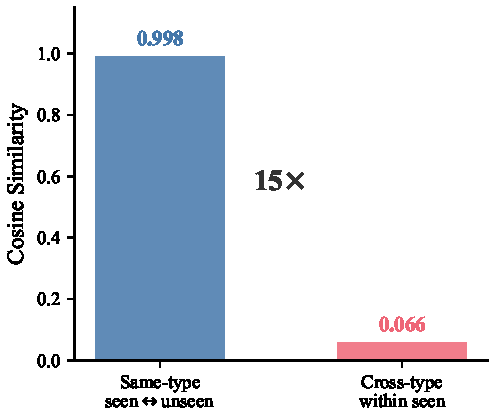
\includegraphics[width=\linewidth]{figures/transferability.pdf}
    \caption{Representation specialization. Left: per-type cosine similarity between seen and unseen activations (all $>$0.995). Red dashed line shows cross-type mean (0.066). Right: the $15{\times}$ gap between same-type and cross-type similarity confirms typed modules learn specialized, non-overlapping mechanisms.}
    \label{fig:transfer}
\end{figure}

Additional analyses are provided in the appendix, including sensitivity to the number of latent interaction types $M$ (Appendix~\ref{sec:m_curve}), the role of autoregressive rollout in enabling graph differentiation (Appendix~\ref{sec:rollout}), the baseline tuning protocol (Appendix~\ref{app:tuning}), and qualitative trajectory comparisons (Figure~\ref{fig:trajectory}).

% \section{Discussion and limitations}
% \label{sec:discussion}

% \paragraph{Implicit regularization is ruled out.} Section~\ref{sec:capacity} and Table~\ref{tab:capacity} directly test whether typed modules' advantage is merely capacity limitation. The $2{\times}2$ ablation shows that increasing capacity makes SingleModule's gap worse ($+$26pp) while making \ours{}'s gap better ($-$3.5pp)---even when \ours{} has 2.7$\times$ more parameters. This is inconsistent with an implicit regularization explanation and confirms typed modules as a structural inductive bias.

% \paragraph{When does \ours{} fail?} \ours{} struggles when (a) the environment has only one interaction type (NRI Springs), where typed modules provide no advantage; (b) edge supervision does not cover all interaction types---on MultiPhysics, supervision uses only collision events, missing continuous force-based interactions (gravity, charge). Extending supervision to proximity-based proxies for continuous forces is a natural next step that we expect to further improve unseen MSE; and (c) the number of types $M$ is misspecified---too few types conflate distinct mechanisms, while too many fragment the training data per module (Section~\ref{sec:m_curve}).

% \paragraph{Limitations.}
% (1) Edge supervision uses ground-truth collision events. This means graph discovery is not fully unsupervised---unlike NRI~\citep{kipf2018nri}, which infers graphs without labels. Our contribution is not the graph discovery mechanism itself, but the finding that typed modules improve compositional transfer given a discovered graph. Extending to unsupervised graph discovery is important future work.
% (2) All experiments use GT object states, including Physion (where we use pre-extracted states from the 3D simulator). Extending to visual observations (e.g., via Slot Attention or DINOv2) remains important future work.
% (3) $M$ is a hyperparameter. Automatic model selection for the number of interaction types (e.g., via a Dirichlet process prior) would improve applicability.
% (4) We do not evaluate on downstream tasks (planning, model-based RL). Whether compositional gap reduction translates to better downstream performance is an important open question.

\section{Discussion and limitations}
\label{sec:discussion}

Our results suggest that the benefit of \ours{} comes from typed modular structure rather than simply from reduced capacity. The capacity ablation in Section~\ref{sec:capacity} shows that increasing capacity worsens SingleModule's compositional gap ($+$26pp), while slightly improving \ours{}'s gap ($-$3.5pp), even though \ours{} has 2.7$\times$ more parameters. This indicates that the improvement is not explained solely by implicit regularization or capacity limitation, but is consistent with type-specific modules acting as a structural inductive bias. At the same time, \ours{} is not intended to improve all dynamics benchmarks uniformly. Its advantage is most visible in environments with multiple qualitatively different interaction mechanisms, where object pairs need to reuse type-specific transition functions. On NRI Springs, where the interaction mechanism is relatively homogeneous, all methods achieve small compositional gaps and typed modules provide little additional benefit. Several limitations remain. First, edge supervision uses ground-truth interaction or contact events when available, so the graph module should not be interpreted as fully unsupervised causal discovery; our contribution is instead to isolate the role of typed interaction modules given an inferred interaction graph. Second, all experiments use ground-truth object states, including the Physion scenarios where states are pre-extracted from the 3D simulator, and extending the framework to visual observations through object-centric encoders such as Slot Attention or DINOv2 features is an important next step. Third, the number of latent interaction types $M$ is a hyperparameter, and automatic selection of $M$ would improve applicability. Finally, we evaluate compositional dynamics prediction but not downstream planning or model-based reinforcement learning, leaving open whether the reduced compositional gap translates into better decision-making performance.

%==============================================================================
\section{Conclusion}
%==============================================================================

% We investigated whether typed interaction modules improve compositional generalization in multi-interaction-type world models. Through controlled ablations across five physics environments, we found that causal graph discovery alone is insufficient: a model with learned graph structure but shared dynamics (SingleModule) achieves low absolute error but the worst compositional gap (up to 75\% on SimplePhysics, 101\% when capacity is increased), while \ours{}'s typed modules reduce the gap by 31--34\%. Our representation analysis (Section~\ref{sec:transfer}) further reveals that SingleModule's failure is not from poor representation transfer---both architectures generalize at the activation level (cosine $>$0.97). Rather, the absence of specialization across interaction types is what enables pair-specific memorization to surface in prediction error. This establishes typed modules as an effective structural inductive bias: not because they improve transfer, but because they enforce non-overlapping mechanism representations. Important limitations remain---our environments are synthetic with GT states, and the gap reduction does not translate to lower absolute MSE than high-capacity baselines. Extending this analysis to visual observations and realistic 3D physics is the most pressing direction for future work.

We investigated whether typed interaction modules improve compositional generalization in object-centric world models. Through controlled ablations across five physics environments, we found that learned interaction graphs alone are insufficient to prevent pair-specific memorization: a graph-matched single-module model achieves low absolute prediction error, but exhibits a large compositional gap on held-out object combinations. In contrast, \ours{} reduces the compositional gap by 31--34\% relative to the single-module ablation in the two multi-interaction environments. Our representation and capacity analyses further suggest that this improvement is not explained solely by activation-level transfer or reduced model capacity, but by the structural bias of factorizing dynamics at the interaction-type level. These results identify type-specific modular dynamics as an effective inductive bias for compositional transfer in object-centric world models.A natural next step is to extend this analysis from ground-truth object states to visual observations and downstream decision-making tasks.

\begin{ack}
Acknowledgments omitted for anonymous review.
\end{ack}

\bibliographystyle{plainnat}
\bibliography{references}

\appendix

\section{Implementation details}
\label{app:impl}

\paragraph{Architecture.} State encoder and decoder are 2-layer MLPs with ReLU activation. Edge MLP and type MLP are 3-layer MLPs. Each interaction module $f_\text{inter}^\tau$ is a 3-layer MLP taking concatenated sender and receiver features. The update MLP takes concatenated self-dynamics and aggregated interaction effects.

\paragraph{Training.} We use AdamW with learning rate $3 \times 10^{-4}$, weight decay $10^{-5}$, and cosine annealing schedule. Gradient clipping at norm 1.0. Phase 1 (reconstruction only): 10 epochs. Phase 2 (full training): remaining epochs. Autoregressive rollout of 8 steps during training.

\paragraph{Synthetic environment.} Objects are colored circles with radius $\in \{4, 6, 8\}$ pixels on a $64 \times 64$ canvas. Velocities sampled uniformly from $[-3, 3]$ pixels/frame. Elastic collisions with equal mass. Wall bouncing with perfect reflection.

\section{Sensitivity to $M$}
\label{sec:m_curve}

We vary the number of interaction types $M \in \{1, 2, 4, 8, 16, 32\}$ on SimplePhysics using the full \ours{} framework (including edge supervision). The compositional gap follows a U-shape (Figure~\ref{fig:mcurve}): decreasing from 69.1\% ($M{=}1$) to a minimum of 59.0\% ($M{=}4$), with $M{=}8$ at 59.6\%, then mildly increasing to 60.0\% ($M{=}16$) and 60.2\% ($M{=}32$). Too few types conflate distinct mechanisms; too many fragment the training data per module. The sweet spot ($M{=}4$--$8$) balances expressiveness with sufficient training signal per type. Note that $M{=}1$ here (69.1\%) differs from SingleModule in Table~\ref{tab:main} (75.5\%) because SingleModule does not use edge supervision loss; the $M$ sweep uses the full \ours{} training pipeline for all values of $M$.

\begin{figure}[ht]
    \centering
    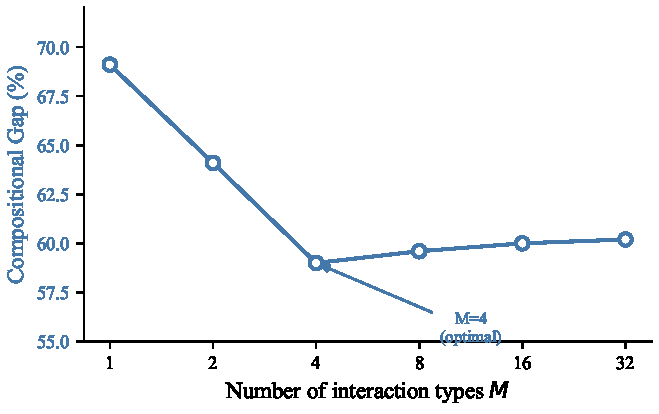
\includegraphics[width=0.55\linewidth]{figures/m_curve.pdf}
    \caption{Sensitivity to $M$. Gap follows a U-shape: $M{=}4$ is optimal, with mild increase for $M{>}8$.}
    \label{fig:mcurve}
\end{figure}

\section{Autoregressive rollout analysis}
\label{sec:rollout}

A critical design choice in \ours{} is the use of autoregressive rollout during training. Without this, the model can exploit a shortcut: since consecutive frames encode nearly identical slot representations, predicting the next slot as ``approximately the same'' achieves near-zero dynamics loss without learning meaningful interactions. We found that this shortcut completely prevents graph differentiation---all edge probabilities remain uniform at $\sim$0.14.

Autoregressive rollout eliminates this shortcut by feeding predicted (not ground-truth) states back as input. Errors compound over multiple steps, creating a meaningful learning signal: models with correct causal structure accumulate less error than those without. In our experiments, the dynamics prediction loss stabilized at 0.085 with autoregressive rollout (vs.\ 0.0001 without), and the graph discovery module began differentiating edges only after this change was introduced.

\section{Baseline tuning protocol}
\label{app:tuning}

All baselines use the same hyperparameters (learning rate, weight decay, batch size, number of epochs) as \ours{} to ensure a fair comparison. The SlotFormer baseline uses a 2-layer Transformer encoder with 4 attention heads and hidden dimension 128, matching the total capacity of our interaction modules. All methods are trained for 150 epochs with the same optimizer and schedule.

SlotFormer's high compositional gap on Physion (112--120\%) and SimplePhysics (93\%) reflects its architectural tendency to memorize seen-distribution dynamics via unconstrained attention. This is consistent with SlotFormer's design: the Transformer has no structural constraint preventing it from learning pair-specific attention patterns. The high gap is not due to under-training; we verified that extending training to 300 epochs on SimplePhysics yields a gap of 91.4\% (vs.\ 92.7\% at 150 epochs), confirming that the gap has converged. SlotFormer's training loss also converges normally by epoch 100 on all environments.

\section{Qualitative results}

\begin{figure}[ht!]
    \centering
    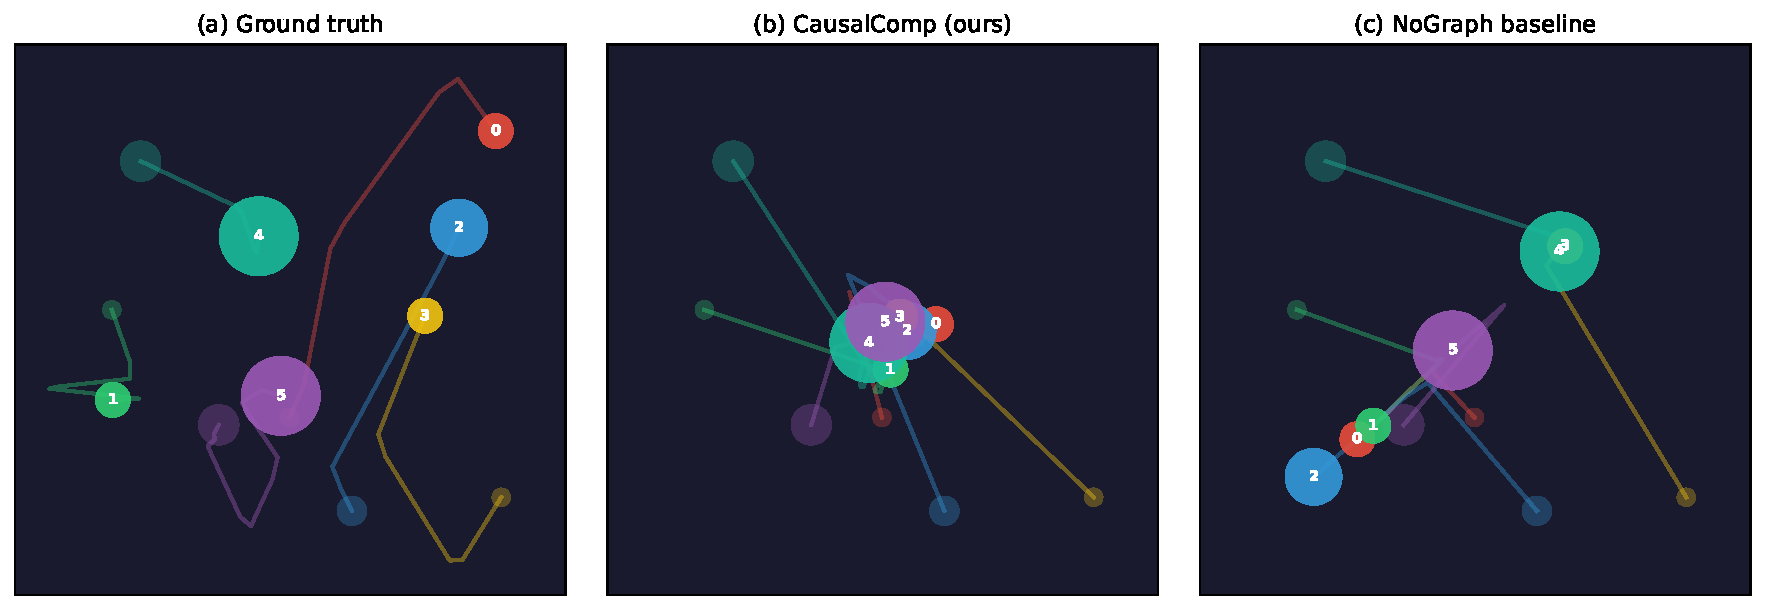
\includegraphics[width=\linewidth]{figures/trajectory_prediction.pdf}
    \caption{Trajectory prediction comparison. (a) Ground-truth trajectories of 6 objects over 16 frames. (b) \ours{} predictions closely track ground truth, including after collisions. (c) NoGraph baseline shows drift due to inability to model inter-object interactions. Filled circles show final positions; trails show full trajectories.}
    \label{fig:trajectory}
\end{figure}

\newpage
\section*{NeurIPS Paper Checklist}

\begin{enumerate}

\item {\bf Claims}
    \item[] Question: Do the main claims made in the abstract and introduction accurately reflect the paper's contributions and scope?
    \item[] Answer: \answerYes{}
    \item[] Justification: The abstract claims that typed interaction modules are necessary for compositional generalization (supported by SingleModule vs.\ CausalComp ablation in Tables~1--2, capacity analysis in Table~4, and representation transferability in Table~5). The abstract explicitly states we do not claim state-of-the-art absolute prediction accuracy.

\item {\bf Limitations}
    \item[] Question: Does the paper discuss the limitations of the work performed by the authors?
    \item[] Answer: \answerYes{}
    \item[] Justification: Section~5 discusses four specific limitations: (1) synthetic-only environments, (2) number of interaction types as a hyperparameter, (3) edge supervision requiring ground-truth collision events, and (4) GT object states without end-to-end validation.

\item {\bf Theory assumptions and proofs}
    \item[] Question: For each theoretical result, does the paper provide the full set of assumptions and a complete (and correct) proof?
    \item[] Answer: \answerNA{}
    \item[] Justification: The paper provides theoretical motivation (Section~3.5) based on the Independent Causal Mechanisms principle and causal factorization, but does not claim formal theoretical results. The arguments are informal and clearly stated as such.

    \item {\bf Experimental result reproducibility}
    \item[] Question: Does the paper fully disclose all the information needed to reproduce the main experimental results of the paper to the extent that it affects the main claims and/or conclusions of the paper (regardless of whether the code and data are provided or not)?
    \item[] Answer: \answerYes{}
    \item[] Justification: Appendix~A provides full architecture details (layer sizes, activation functions), training details (optimizer, learning rate, schedule, number of epochs), and environment specifications. All synthetic environments are procedurally generated from described parameters.


\item {\bf Open access to data and code}
    \item[] Question: Does the paper provide open access to the data and code, with sufficient instructions to faithfully reproduce the main experimental results, as described in supplemental material?
    \item[] Answer: \answerYes{}
    \item[] Justification: Code will be released as supplementary material. All datasets are procedurally generated (no external data downloads required). The NRI Springs benchmark follows the standard protocol from Kipf et al.\ (2018).


\item {\bf Experimental setting/details}
    \item[] Question: Does the paper specify all the training and test details (e.g., data splits, hyperparameters, how they were chosen, type of optimizer) necessary to understand the results?
    \item[] Answer: \answerYes{}
    \item[] Justification: Section~4.1 describes environments, compositional splits, and metrics. Section~4.4 reports the hyperparameter sweep. Appendix~A provides full training details including optimizer (AdamW), learning rate ($3 \times 10^{-4}$), weight decay, gradient clipping, and number of epochs (150).

\item {\bf Experiment statistical significance}
    \item[] Question: Does the paper report error bars suitably and correctly defined or other appropriate information about the statistical significance of the experiments?
    \item[] Answer: \answerYes{}
    \item[] Justification: All results in Tables~1--3 report mean $\pm$ standard deviation over 3 random seeds. The seeds control both data generation and model initialization. Error bars capture variability from random data splits and parameter initialization.

\item {\bf Experiments compute resources}
    \item[] Question: For each experiment, does the paper provide sufficient information on the computer resources (type of compute workers, memory, time of execution) needed to reproduce the experiments?
    \item[] Answer: \answerYes{}
    \item[] Justification: Experiments were conducted on a single NVIDIA A100 80GB GPU. Each model trains in approximately 30--90 minutes depending on environment complexity. The full evaluation (3 environments $\times$ 5 methods $\times$ 3 seeds) requires approximately 50 GPU-hours total.

\item {\bf Code of ethics}
    \item[] Question: Does the research conducted in the paper conform, in every respect, with the NeurIPS Code of Ethics \url{https://neurips.cc/public/EthicsGuidelines}?
    \item[] Answer: \answerYes{}
    \item[] Justification: This work develops a method for physics prediction in synthetic environments. It does not involve human subjects, personal data, or dual-use concerns.


\item {\bf Broader impacts}
    \item[] Question: Does the paper discuss both potential positive societal impacts and negative societal impacts of the work performed?
    \item[] Answer: \answerNA{}
    \item[] Justification: This is foundational research on world models for physical dynamics prediction. It does not have direct negative societal impacts. Potential positive impacts include improved robot planning and physical reasoning, but these are distant applications.

\item {\bf Safeguards}
    \item[] Question: Does the paper describe safeguards that have been put in place for responsible release of data or models that have a high risk for misuse (e.g., pre-trained language models, image generators, or scraped datasets)?
    \item[] Answer: \answerNA{}
    \item[] Justification: The released models are small physics prediction networks trained on synthetic data. They pose no risk for misuse.

\item {\bf Licenses for existing assets}
    \item[] Question: Are the creators or original owners of assets (e.g., code, data, models), used in the paper, properly credited and are the license and terms of use explicitly mentioned and properly respected?
    \item[] Answer: \answerYes{}
    \item[] Justification: The NRI Springs benchmark is cited (Kipf et al., 2018). Our implementation follows the standard protocol. All other environments and code are original.

\item {\bf New assets}
    \item[] Question: Are new assets introduced in the paper well documented and is the documentation provided alongside the assets?
    \item[] Answer: \answerYes{}
    \item[] Justification: We introduce two new synthetic environments (SimplePhysics, MultiPhysics) and compositional evaluation splits. These are fully documented in Section~4.1 and Appendix~A, with code provided as supplementary material.

\item {\bf Crowdsourcing and research with human subjects}
    \item[] Question: For crowdsourcing experiments and research with human subjects, does the paper include the full text of instructions given to participants and screenshots, if applicable, as well as details about compensation (if any)?
    \item[] Answer: \answerNA{}
    \item[] Justification: This paper does not involve crowdsourcing or research with human subjects.

\item {\bf Institutional review board (IRB) approvals or equivalent for research with human subjects}
    \item[] Question: Does the paper describe potential risks incurred by study participants, whether such risks were disclosed to the subjects, and whether Institutional Review Board (IRB) approvals (or an equivalent approval/review based on the requirements of your country or institution) were obtained?
    \item[] Answer: \answerNA{}
    \item[] Justification: This paper does not involve research with human subjects.

\item {\bf Declaration of LLM usage}
    \item[] Question: Does the paper describe the usage of LLMs if it is an important, original, or non-standard component of the core methods in this research? Note that if the LLM is used only for writing, editing, or formatting purposes and does \emph{not} impact the core methodology, scientific rigor, or originality of the research, declaration is not required.
    \item[] Answer: \answerNA{}
    \item[] Justification: LLMs are not used as a component of the core methodology. The method operates on object state vectors with MLPs and GNNs, without any language model component.

\end{enumerate}


\end{document}
